
\documentclass[a4paper,12pt]{article}
%%%%%%%%%%%%%%%%%%%%%%%%%%%%%%%%%%%%%%%%%%%%%%%%%%%%%%%%%%%%%%%%%%%%%%%%%%%%%%%%%%%%%%%%%%%%%%%%%%%%%%%%%%%%%%%%%%%%%%%%%%%%%%%%%%%%%%%%%%%%%%%%%%%%%%%%%%%%%%%%%%%%%%%%%%%%%%%%%%%%%%%%%%%%%%%%%%%%%%%%%%%%%%%%%%%%%%%%%%%%%%%%%%%%%%%%%%%%%%%%%%%%%%%%%%%%
\usepackage{eurosym}
\usepackage{vmargin}
\usepackage{amsmath}
\usepackage{graphics}
\usepackage{epsfig}
\usepackage{framed}
\usepackage{subfigure}
\usepackage{fancyhdr}
\usepackage{framed}
\usepackage{subfiles}
\usepackage{graphics}
\usepackage{newlfont}
\usepackage{eurosym}
\usepackage{amsmath,amsthm,amsfonts}
\usepackage{amsmath}
\usepackage{enumerate}
\usepackage{color}
\usepackage{multicol}
\usepackage{amssymb}
\usepackage{multicol}
\usepackage[dvipsnames]{xcolor}
\usepackage{graphicx}

\setcounter{MaxMatrixCols}{10}
%TCIDATA{OutputFilter=LATEX.DLL}
%TCIDATA{Version=5.00.0.2570}
%TCIDATA{<META NAME="SaveForMode"CONTENT="1">}
%TCIDATA{LastRevised=Wednesday, February 23, 201113:24:34}
%TCIDATA{<META NAME="GraphicsSave" CONTENT="32">}
%TCIDATA{Language=American English}

\pagestyle{fancy}
\setmarginsrb{20mm}{0mm}{20mm}{25mm}{12mm}{11mm}{0mm}{11mm}
\lhead{MA4128} \rhead{Kevin O'Brien} \chead{Binary Classification} %\input{tcilatex}

%http://www.electronics.dit.ie/staff/ysemenova/Opto2/CO_IntroLab.pdf
\begin{document}
\section{SPSS Implementation and Output}

Hierarchical Cluster Analysis is implemented by the \textbf{classify} option on the \textbf{analyse} menu.
Three options shall appear. Select Hierarchical.

We performed a hierarchical cluster analysis in SPSS, selecting all the variables (except categorical variables) in the \textbf{Variable(s)} box. We can label the cases by a categorical variable. 

We shall further requested the Dendrogram in the output. We changed all
variables to z-scores to yield equal metrics and equal weighting, selected the Squared Euclidean distance
(the default) method of determining distance between clusters and the \textbf{Ward's method} for
clustering, and saved a 3-cluster solution as a new variable.

\subsection{Proximity matrix}
The output will print distances or similarities computed for any pair of cases. We will not be covering this in detail.

\subsection{Cluster Membership}
This box allows you to specify a set number of clusters. If you have a
hypothesis about how many clusters there are, you can specify a set number of clusters, or
create a number of clusters within a range.

\subsection{Icicle Plot} Default choice by SPSS. Icicle plots visually represent information on the agglomeration
schedule. You can select that all clusters are included in the icicle plot, or restrict it to a range of
clusters. Also, you can read the plot from bottom up (vertical orientation) or from left to right
(horizontal orientation).

\subsection{Measure} There are different distance measure choices depending on the level of measurement
of the data: interval, count, or binary.
For nearly all of this module example,the data were on an interval scale, and the squared euclidean measure will suffice.


\newpage
\subsection{SPSS Agglomeration Schedule}
\begin{center}
	\begin{figure}
		% Requires \usepackage{graphicx}
		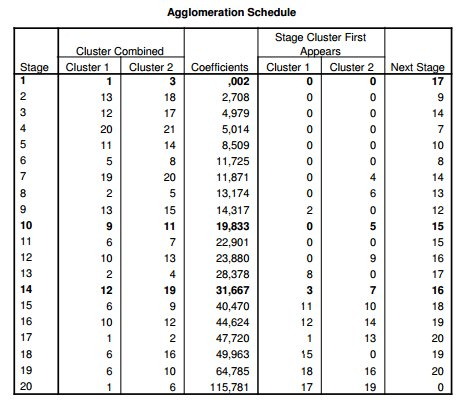
\includegraphics[scale=1.1]{images/AggloSc}\\
		%\caption{SPSS Agglomeration Schedule}
	\end{figure}
\end{center}


The procedure followed by cluster analysis at Stage 1 is to cluster the two cases that have the smallest
squared Euclidean distance between them. Then SPSS will recompute the distance measures between all
single cases and clusters (there is only one cluster of two cases after the first step). Next, the 2 cases (or
clusters) with the smallest distance will be combined, yielding either 2 clusters of 2 cases (with 17 cases
unclustered) or one cluster of 3 (with 18 cases unclustered).  This process continues until all cases are clustered into a single group.
For the sake of clarify, we will explain Stages 1, 10, and 14.


\subsubsection{Stage 1}
At Stage 1, Case 1 is clustered with Case 3. The squared Euclidean distance between these two cases is
.002. Neither variable has been previously clustered (the two zeros under Cluster 1 and Cluster 2), and the
next stage (when the cluster containing Case 1 combines with another case) is Stage 17. (Note that at Stage
17, Case 2 joins the Case-1 cluster.)

\subsubsection{Stage 10}
\begin{itemize}
	\item At Stage 10, Case 9 joins the Case-11 cluster (Case 11 was previously clustered with Case 14 back in Stage
	5, thus creating a cluster of 3 cases: Cases 9, 11, and 14). 
	\item The squared Euclidean distance between Case 9
	and Case-11 cluster is 19.833. 
	\item Case 9 has not been previously clustered (the zero under Cluster 1), and
	Case 11 was previously clustered at Stage 5. 
	\item The next stage (when the cluster containing Case 9 clusters) is
	Stage 15 (when it combines with the Case-6 cluster).
\end{itemize}


\subsubsection{Stage 14}
\begin{itemize}
	\item At Stage 14, the clusters containing Cases 12 and 19 are joined, Case 12 has been previously clustered with
	Case 17, and Case 19 had been previously clustered with Cases 20 and 21, thus forming a cluster of 5 cases
	(Cases 12, 17, 19, 20, 21). 
	\item The squared Euclidean distance between the two joined clusters is 31.667. 
	\item Case
	12 was previously joined at Stage 3 with Case 17. Case 19 was previously joined at Stage 7 with the Case-
	20 cluster. 
	\item The next stage when the Case-12 cluster will combine with another case/cluster is Stage 16
	(when it joins with the Case-10 cluster).
\end{itemize}


\begin{figure}
	% Requires \usepackage{graphicx}
	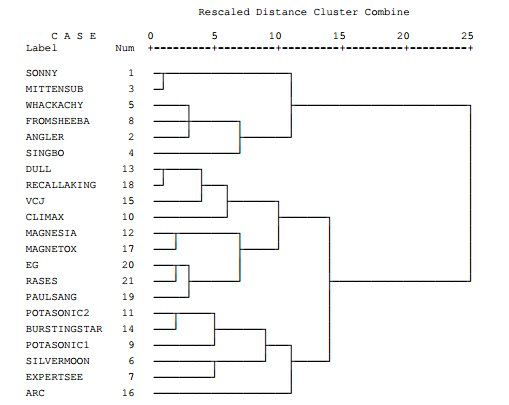
\includegraphics[scale=1.0]{images/Dendro}\\
	\caption{Corresponding Dendrogram}
\end{figure}

The branching-type nature of the Dendrogram allows you to trace backward or forward to any individual
case or cluster at any level. It, in addition, gives an idea of how great the distance was between cases or
groups that are clustered in a particular step, using a 0 to 25 scale along the top of the chart. While it is
difficult to interpret distance in the early clustering phases (the extreme left of the graph), as you move to
the right relative distance become more apparent. The bigger the distances before two clusters are joined,
the bigger the differences in these clusters. To find a membership of a particular cluster simply trace
backwards down the branches to the name.

%----------------------------------------------------- %
\newpage
\section{Non-Hierarchical Clustering}
This method of clustering is very different from the hierarchical clustering and Ward method, which are applied when there is no prior knowledge of how many clusters there may be or what they are characterized by. The k-means clustering approach is used when you already have hypotheses concerning the number of clusters in your cases or variables. For example, you may want to specify exactly three clusters that are to be as distinct as possible.

This is the type of research question that can be addressed by the k-means clustering algorithm. In general, the k-means method will produce the exact k different clusters demanded of greatest possible distinction. Very often, both the hierarchical and the k-means techniques are used successively.
\begin{itemize}
	\item Ward's method is used to get some sense of the possible number of clusters and the way they merge as seen from the dendrogram.
	\item Then the clustering is rerun with only a chosen optimum number in which to place all
	the cases (i.e. k means clustering).
\end{itemize}

In these methods the desired number of clusters is specified in advance and the `best' solution
is chosen. The steps in such a method are as follows:
\begin{itemize}
	\item[1] Choose initial cluster centres (essentially this is a set of observations that are far apart
	— each subject forms a cluster of one and its centre is the value of the variables for
	that subject).
	\item[2] Assign each subject to its `nearest' cluster, defined in terms of the distance to the
	centroid.
	\item[3] Find the centroids of the clusters that have been formed
	\item[4] Re-calculate the distance from each subject to each centroid and move observations that
	are not in the cluster that they are closest to.
	\item[5] Continue until the centroids remain relatively stable.
\end{itemize}

Non-hierarchical cluster analysis tends to be used when large data sets are involved. It is
sometimes preferred because it allows subjects to move from one cluster to another (this is
not possible in hierarchical cluster analysis where a subject, once assigned, cannot move to a
different cluster). Two disadvantages of non-hierarchical cluster analysis are: 
\begin{itemize}
	\item[1]it is often
	diffcult to know how many clusters you are likely to have and therefore the analysis may have
	to be repeated several times 
	\item[2] it can be very sensitive to the choice of initial cluster centres. Again, it may be worth trying di?erent ones to see what impact this has.
\end{itemize}

\subsection{Optimal Number of Clusters}
One of the biggest problems with cluster analysis is identifying the optimum number of
clusters. As the joining process continues, increasingly dissimilar clusters must be joined. i.e. the classification becomes increasingly artificial. Deciding upon the optimum number
of clusters is largely subjective, although looking at a dendrogram would help.

% http://www.uk.sagepub.com/burns/data.htm
% Data Set 23 A

% DASL
% http://lib.stat.cmu.edu/cgi-bin/dasl.cgi?query=Cluster+analysis&submit=Search%21&metaname=methods&sort=swishrank

\end{document}